\documentclass[1p]{elsarticle_modified}
%\bibliographystyle{elsarticle-num}

%\usepackage[colorlinks]{hyperref}
%\usepackage{abbrmath_seonhwa} %\Abb, \Ascr, \Acal ,\Abf, \Afrak
\usepackage{amsfonts}
\usepackage{amssymb}
\usepackage{amsmath}
\usepackage{amsthm}
\usepackage{scalefnt}
\usepackage{amsbsy}
\usepackage{kotex}
\usepackage{caption}
\usepackage{subfig}
\usepackage{color}
\usepackage{graphicx}
\usepackage{xcolor} %% white, black, red, green, blue, cyan, magenta, yellow
\usepackage{float}
\usepackage{setspace}
\usepackage{hyperref}

\usepackage{tikz}
\usetikzlibrary{arrows}

\usepackage{multirow}
\usepackage{array} % fixed length table
\usepackage{hhline}

%%%%%%%%%%%%%%%%%%%%%
\makeatletter
\renewcommand*\env@matrix[1][\arraystretch]{%
	\edef\arraystretch{#1}%
	\hskip -\arraycolsep
	\let\@ifnextchar\new@ifnextchar
	\array{*\c@MaxMatrixCols c}}
\makeatother %https://tex.stackexchange.com/questions/14071/how-can-i-increase-the-line-spacing-in-a-matrix
%%%%%%%%%%%%%%%

\usepackage[normalem]{ulem}

\newcommand{\msout}[1]{\ifmmode\text{\sout{\ensuremath{#1}}}\else\sout{#1}\fi}
%SOURCE: \msout is \stkout macro in https://tex.stackexchange.com/questions/20609/strikeout-in-math-mode

\newcommand{\cancel}[1]{
	\ifmmode
	{\color{red}\msout{#1}}
	\else
	{\color{red}\sout{#1}}
	\fi
}

\newcommand{\add}[1]{
	{\color{blue}\uwave{#1}}
}

\newcommand{\replace}[2]{
	\ifmmode
	{\color{red}\msout{#1}}{\color{blue}\uwave{#2}}
	\else
	{\color{red}\sout{#1}}{\color{blue}\uwave{#2}}
	\fi
}

\newcommand{\Sol}{\mathcal{S}} %segment
\newcommand{\D}{D} %diagram
\newcommand{\A}{\mathcal{A}} %arc


%%%%%%%%%%%%%%%%%%%%%%%%%%%%%5 test

\def\sl{\operatorname{\textup{SL}}(2,\Cbb)}
\def\psl{\operatorname{\textup{PSL}}(2,\Cbb)}
\def\quan{\mkern 1mu \triangleright \mkern 1mu}

\theoremstyle{definition}
\newtheorem{thm}{Theorem}[section]
\newtheorem{prop}[thm]{Proposition}
\newtheorem{lem}[thm]{Lemma}
\newtheorem{ques}[thm]{Question}
\newtheorem{cor}[thm]{Corollary}
\newtheorem{defn}[thm]{Definition}
\newtheorem{exam}[thm]{Example}
\newtheorem{rmk}[thm]{Remark}
\newtheorem{alg}[thm]{Algorithm}

\newcommand{\I}{\sqrt{-1}}
\begin{document}

%\begin{frontmatter}
%
%\title{Boundary parabolic representations of knots up to 8 crossings}
%
%%% Group authors per affiliation:
%\author{Yunhi Cho} 
%\address{Department of Mathematics, University of Seoul, Seoul, Korea}
%\ead{yhcho@uos.ac.kr}
%
%
%\author{Seonhwa Kim} %\fnref{s_kim}}
%\address{Center for Geometry and Physics, Institute for Basic Science, Pohang, 37673, Korea}
%\ead{ryeona17@ibs.re.kr}
%
%\author{Hyuk Kim}
%\address{Department of Mathematical Sciences, Seoul National University, Seoul 08826, Korea}
%\ead{hyukkim@snu.ac.kr}
%
%\author{Seokbeom Yoon}
%\address{Department of Mathematical Sciences, Seoul National University, Seoul, 08826,  Korea}
%\ead{sbyoon15@snu.ac.kr}
%
%\begin{abstract}
%We find all boundary parabolic representation of knots up to 8 crossings.
%
%\end{abstract}
%\begin{keyword}
%    \MSC[2010] 57M25 
%\end{keyword}
%
%\end{frontmatter}

%\linenumbers
%\tableofcontents
%
\newcommand\colored[1]{\textcolor{white}{\rule[-0.35ex]{0.8em}{1.4ex}}\kern-0.8em\color{red} #1}%
%\newcommand\colored[1]{\textcolor{white}{ #1}\kern-2.17ex	\textcolor{white}{ #1}\kern-1.81ex	\textcolor{white}{ #1}\kern-2.15ex\color{red}#1	}

{\Large $\underline{12n_{0305}~(K12n_{0305})}$}

\setlength{\tabcolsep}{10pt}
\renewcommand{\arraystretch}{1.6}
\vspace{1cm}\begin{tabular}{m{100pt}>{\centering\arraybackslash}m{274pt}}
\multirow{5}{120pt}{
	\centering
	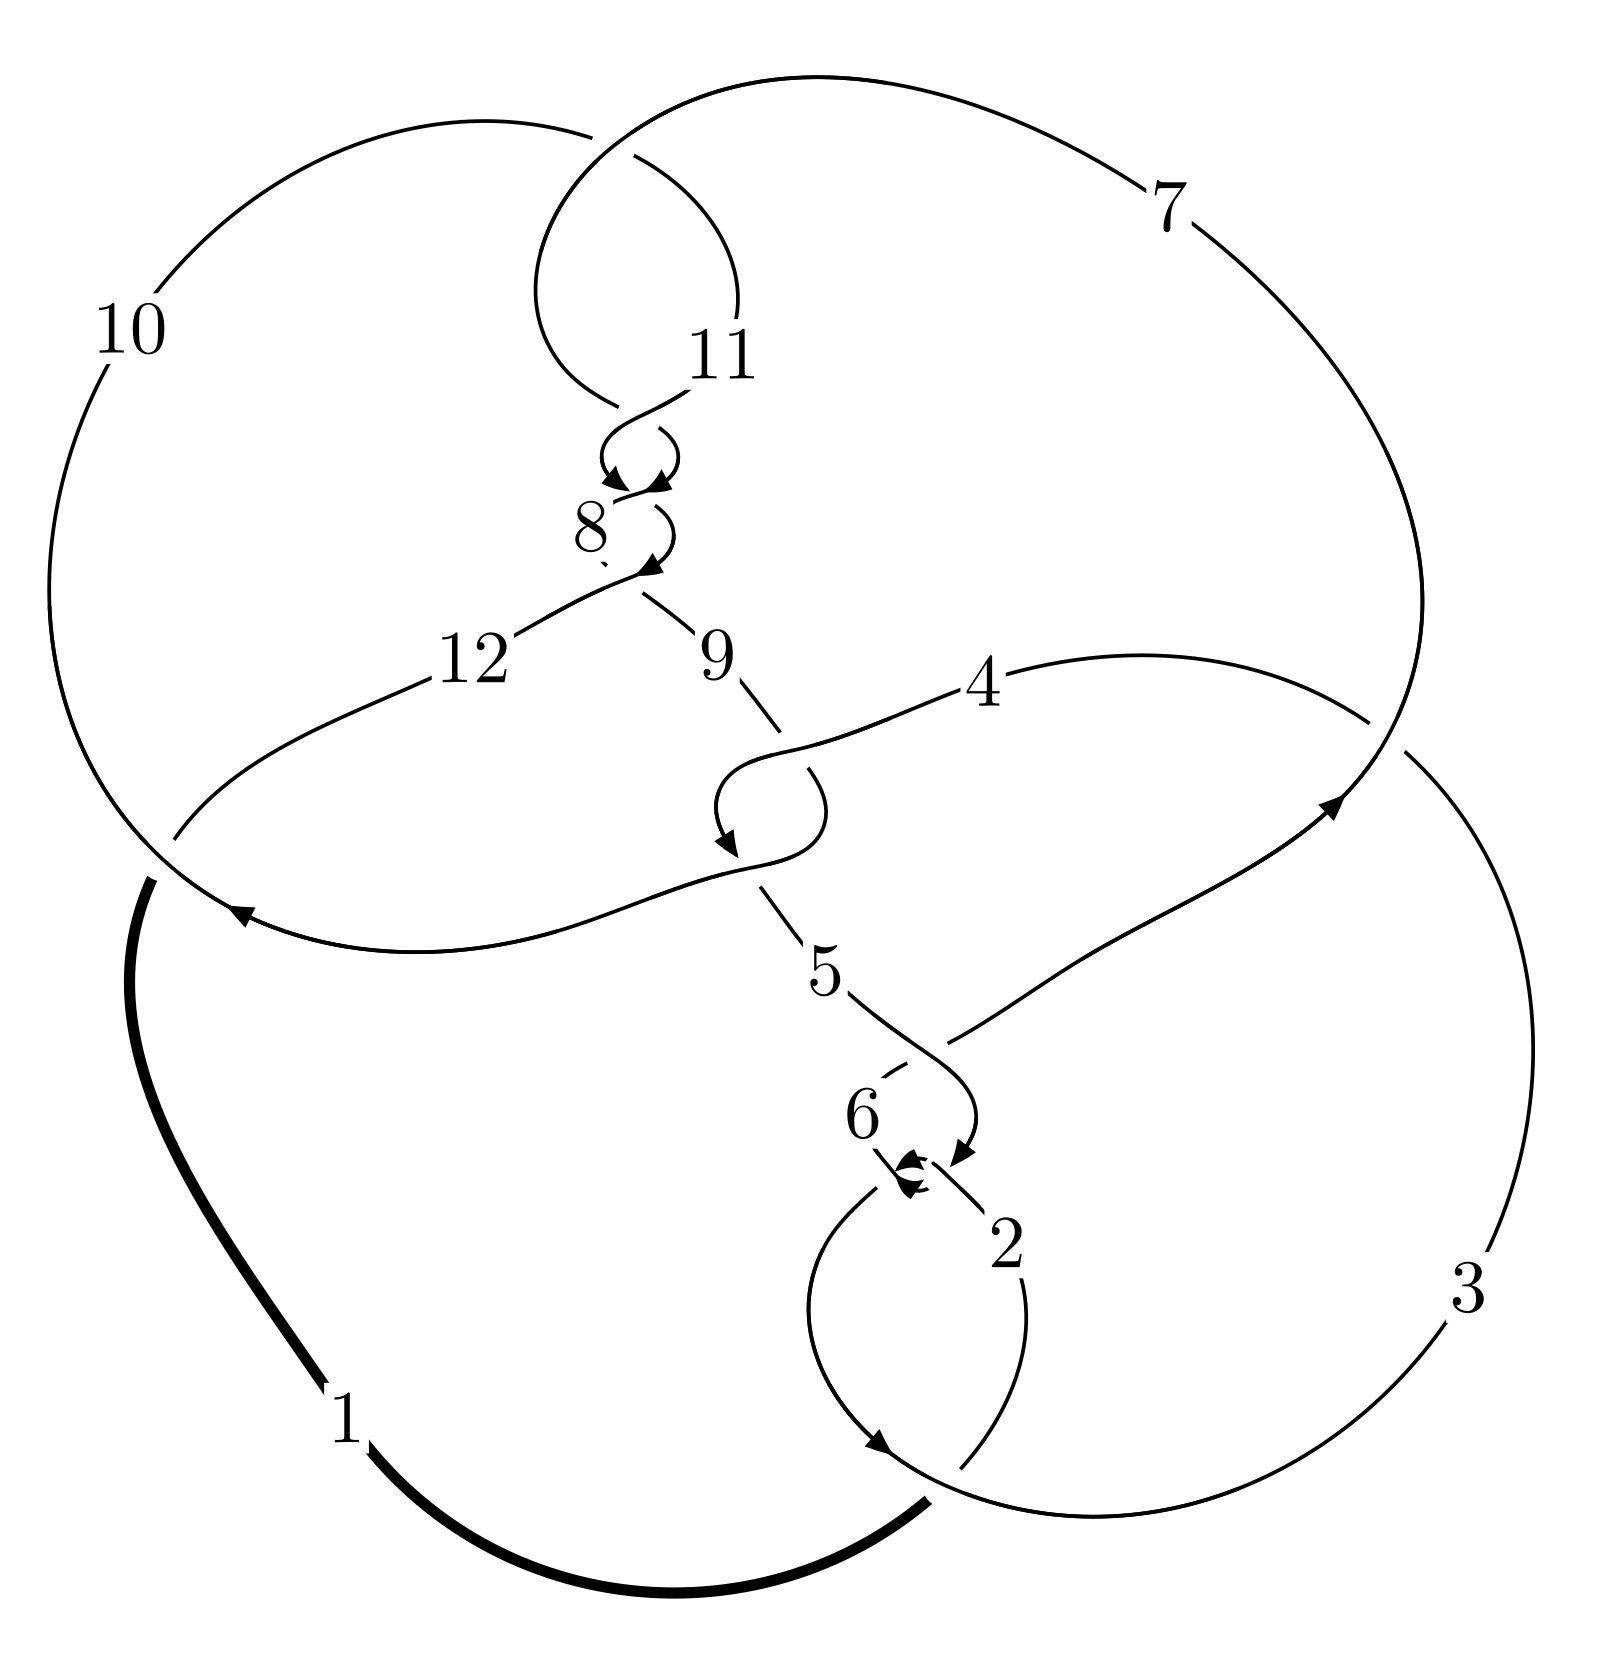
\includegraphics[width=112pt]{../../../GIT/diagram.site/Diagrams/png/2394_12n_0305.png}\\
\ \ \ A knot diagram\footnotemark}&
\allowdisplaybreaks
\textbf{Linearized knot diagam} \\
\cline{2-2}
 &
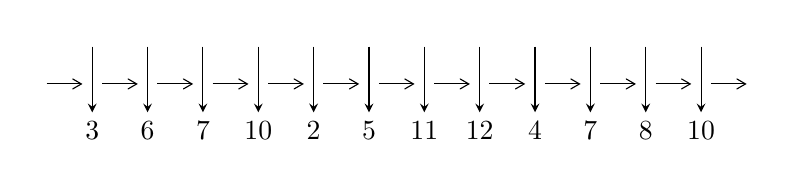
\begin{tikzpicture}[x=20pt, y=17pt]
	% nodes
	\node (C0) at (0, 0) {};
	\node (C1) at (1, 0) {};
	\node (C1U) at (1, +1) {};
	\node (C1D) at (1, -1) {3};

	\node (C2) at (2, 0) {};
	\node (C2U) at (2, +1) {};
	\node (C2D) at (2, -1) {6};

	\node (C3) at (3, 0) {};
	\node (C3U) at (3, +1) {};
	\node (C3D) at (3, -1) {7};

	\node (C4) at (4, 0) {};
	\node (C4U) at (4, +1) {};
	\node (C4D) at (4, -1) {10};

	\node (C5) at (5, 0) {};
	\node (C5U) at (5, +1) {};
	\node (C5D) at (5, -1) {2};

	\node (C6) at (6, 0) {};
	\node (C6U) at (6, +1) {};
	\node (C6D) at (6, -1) {5};

	\node (C7) at (7, 0) {};
	\node (C7U) at (7, +1) {};
	\node (C7D) at (7, -1) {11};

	\node (C8) at (8, 0) {};
	\node (C8U) at (8, +1) {};
	\node (C8D) at (8, -1) {12};

	\node (C9) at (9, 0) {};
	\node (C9U) at (9, +1) {};
	\node (C9D) at (9, -1) {4};

	\node (C10) at (10, 0) {};
	\node (C10U) at (10, +1) {};
	\node (C10D) at (10, -1) {7};

	\node (C11) at (11, 0) {};
	\node (C11U) at (11, +1) {};
	\node (C11D) at (11, -1) {8};

	\node (C12) at (12, 0) {};
	\node (C12U) at (12, +1) {};
	\node (C12D) at (12, -1) {10};
	\node (C13) at (13, 0) {};

	% arrows
	\draw[->,>={angle 60}]
	(C0) edge (C1) (C1) edge (C2) (C2) edge (C3) (C3) edge (C4) (C4) edge (C5) (C5) edge (C6) (C6) edge (C7) (C7) edge (C8) (C8) edge (C9) (C9) edge (C10) (C10) edge (C11) (C11) edge (C12) (C12) edge (C13) ;	\draw[->,>=stealth]
	(C1U) edge (C1D) (C2U) edge (C2D) (C3U) edge (C3D) (C4U) edge (C4D) (C5U) edge (C5D) (C6U) edge (C6D) (C7U) edge (C7D) (C8U) edge (C8D) (C9U) edge (C9D) (C10U) edge (C10D) (C11U) edge (C11D) (C12U) edge (C12D) ;
	\end{tikzpicture} \\
\hhline{~~} \\& 
\textbf{Solving Sequence} \\ \cline{2-2} 
 &
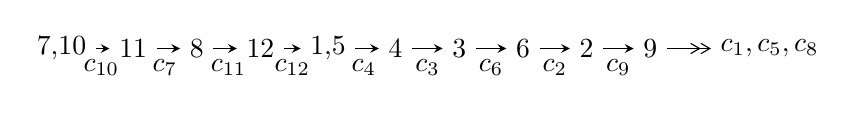
\begin{tikzpicture}[x=23pt, y=7pt]
	% node
	\node (A0) at (-1/8, 0) {7,10};
	\node (A1) at (1, 0) {11};
	\node (A2) at (2, 0) {8};
	\node (A3) at (3, 0) {12};
	\node (A4) at (65/16, 0) {1,5};
	\node (A5) at (41/8, 0) {4};
	\node (A6) at (49/8, 0) {3};
	\node (A7) at (57/8, 0) {6};
	\node (A8) at (65/8, 0) {2};
	\node (A9) at (73/8, 0) {9};
	\node (C1) at (1/2, -1) {$c_{10}$};
	\node (C2) at (3/2, -1) {$c_{7}$};
	\node (C3) at (5/2, -1) {$c_{11}$};
	\node (C4) at (7/2, -1) {$c_{12}$};
	\node (C5) at (37/8, -1) {$c_{4}$};
	\node (C6) at (45/8, -1) {$c_{3}$};
	\node (C7) at (53/8, -1) {$c_{6}$};
	\node (C8) at (61/8, -1) {$c_{2}$};
	\node (C9) at (69/8, -1) {$c_{9}$};
	\node (A10) at (11, 0) {$c_{1},c_{5},c_{8}$};

	% edge
	\draw[->,>=stealth]	
	(A0) edge (A1) (A1) edge (A2) (A2) edge (A3) (A3) edge (A4) (A4) edge (A5) (A5) edge (A6) (A6) edge (A7) (A7) edge (A8) (A8) edge (A9) ;
	\draw[->>,>={angle 60}]	
	(A9) edge (A10);
\end{tikzpicture} \\ 

\end{tabular} \\

\footnotetext{
The image of knot diagram is generated by the software ``\textbf{Draw programme}" developed by Andrew Bartholomew(\url{http://www.layer8.co.uk/maths/draw/index.htm\#Running-draw}), where we modified some parts for our purpose(\url{https://github.com/CATsTAILs/LinksPainter}).
}\phantom \\ \newline 
\centering \textbf{Ideals for irreducible components\footnotemark of $X_{\text{par}}$} 
 
\begin{align*}
I^u_{1}&=\langle 
-3 u^{19}-6 u^{18}+\cdots+2 b-3,\;- u^{19}-12 u^{18}+\cdots+4 a+11,\;u^{20}+4 u^{19}+\cdots+2 u+1\rangle \\
I^u_{2}&=\langle 
b,\;a^3- a^2 u+a^2-2 a u+4 a-2 u+3,\;u^2- u-1\rangle \\
\\
\end{align*}
\raggedright * 2 irreducible components of $\dim_{\mathbb{C}}=0$, with total 26 representations.\\
\footnotetext{All coefficients of polynomials are rational numbers. But the coefficients are sometimes approximated in decimal forms when there is not enough margin.}
\newpage
\renewcommand{\arraystretch}{1}
\centering \section*{I. $I^u_{1}= \langle -3 u^{19}-6 u^{18}+\cdots+2 b-3,\;- u^{19}-12 u^{18}+\cdots+4 a+11,\;u^{20}+4 u^{19}+\cdots+2 u+1 \rangle$}
\flushleft \textbf{(i) Arc colorings}\\
\begin{tabular}{m{7pt} m{180pt} m{7pt} m{180pt} }
\flushright $a_{7}=$&$\begin{pmatrix}0\\u\end{pmatrix}$ \\
\flushright $a_{10}=$&$\begin{pmatrix}1\\0\end{pmatrix}$ \\
\flushright $a_{11}=$&$\begin{pmatrix}1\\u^2\end{pmatrix}$ \\
\flushright $a_{8}=$&$\begin{pmatrix}- u\\- u^3+u\end{pmatrix}$ \\
\flushright $a_{12}=$&$\begin{pmatrix}- u^2+1\\- u^4+2 u^2\end{pmatrix}$ \\
\flushright $a_{1}=$&$\begin{pmatrix}u^4-3 u^2+1\\- u^4+2 u^2\end{pmatrix}$ \\
\flushright $a_{5}=$&$\begin{pmatrix}\frac{1}{4} u^{19}+3 u^{18}+\cdots-15 u-\frac{11}{4}\\\frac{3}{2} u^{19}+3 u^{18}+\cdots+2 u+\frac{3}{2}\end{pmatrix}$ \\
\flushright $a_{4}=$&$\begin{pmatrix}\frac{7}{4} u^{19}+6 u^{18}+\cdots-13 u-\frac{5}{4}\\\frac{3}{2} u^{19}+3 u^{18}+\cdots+2 u+\frac{3}{2}\end{pmatrix}$ \\
\flushright $a_{3}=$&$\begin{pmatrix}\frac{7}{4} u^{19}+6 u^{18}+\cdots-13 u-\frac{5}{4}\\-\frac{5}{4} u^{19}-\frac{11}{4} u^{18}+\cdots+\frac{7}{4} u+\frac{1}{2}\end{pmatrix}$ \\
\flushright $a_{6}=$&$\begin{pmatrix}-\frac{1}{4} u^{18}-\frac{3}{4} u^{17}+\cdots-\frac{21}{4} u-\frac{3}{4}\\u^6-4 u^4+3 u^2+2 u\end{pmatrix}$ \\
\flushright $a_{2}=$&$\begin{pmatrix}\frac{1}{4} u^{18}+\frac{3}{4} u^{17}+\cdots+\frac{17}{4} u+\frac{7}{4}\\\frac{1}{4} u^{19}+\frac{1}{2} u^{18}+\cdots-\frac{1}{2} u+\frac{1}{4}\end{pmatrix}$ \\
\flushright $a_{9}=$&$\begin{pmatrix}u^3-2 u\\u^5-3 u^3+u\end{pmatrix}$\\&\end{tabular}
\flushleft \textbf{(ii) Obstruction class $= -1$}\\~\\
\flushleft \textbf{(iii) Cusp Shapes $= -2 u^{19}-8 u^{18}+16 u^{17}+\frac{191}{2} u^{16}-22 u^{15}-\frac{943}{2} u^{14}-192 u^{13}+\frac{2425}{2} u^{12}+\frac{1981}{2} u^{11}-1627 u^{10}-2079 u^9+\frac{1641}{2} u^8+2156 u^7+431 u^6-908 u^5-571 u^4-\frac{53}{2} u^3+72 u^2+29 u-\frac{21}{2}$}\\~\\
\newpage\renewcommand{\arraystretch}{1}
\flushleft \textbf{(iv) u-Polynomials at the component}\newline \\
\begin{tabular}{m{50pt}|m{274pt}}
Crossings & \hspace{64pt}u-Polynomials at each crossing \\
\hline $$\begin{aligned}c_{1},c_{6}\end{aligned}$$&$\begin{aligned}
&u^{20}+9 u^{19}+\cdots+21 u+1
\end{aligned}$\\
\hline $$\begin{aligned}c_{2},c_{5}\end{aligned}$$&$\begin{aligned}
&u^{20}+3 u^{19}+\cdots-7 u-1
\end{aligned}$\\
\hline $$\begin{aligned}c_{3}\end{aligned}$$&$\begin{aligned}
&u^{20}-3 u^{19}+\cdots-17 u-1
\end{aligned}$\\
\hline $$\begin{aligned}c_{4},c_{9}\end{aligned}$$&$\begin{aligned}
&u^{20}- u^{19}+\cdots-224 u-64
\end{aligned}$\\
\hline $$\begin{aligned}c_{7},c_{8},c_{10}\\c_{11}\end{aligned}$$&$\begin{aligned}
&u^{20}+4 u^{19}+\cdots+2 u+1
\end{aligned}$\\
\hline $$\begin{aligned}c_{12}\end{aligned}$$&$\begin{aligned}
&u^{20}-20 u^{19}+\cdots-3324 u-239
\end{aligned}$\\
\hline
\end{tabular}\\~\\
\newpage\renewcommand{\arraystretch}{1}
\flushleft \textbf{(v) Riley Polynomials at the component}\newline \\
\begin{tabular}{m{50pt}|m{274pt}}
Crossings & \hspace{64pt}Riley Polynomials at each crossing \\
\hline $$\begin{aligned}c_{1},c_{6}\end{aligned}$$&$\begin{aligned}
&y^{20}+7 y^{19}+\cdots-221 y+1
\end{aligned}$\\
\hline $$\begin{aligned}c_{2},c_{5}\end{aligned}$$&$\begin{aligned}
&y^{20}-9 y^{19}+\cdots-21 y+1
\end{aligned}$\\
\hline $$\begin{aligned}c_{3}\end{aligned}$$&$\begin{aligned}
&y^{20}-53 y^{19}+\cdots-69 y+1
\end{aligned}$\\
\hline $$\begin{aligned}c_{4},c_{9}\end{aligned}$$&$\begin{aligned}
&y^{20}-35 y^{19}+\cdots-5120 y+4096
\end{aligned}$\\
\hline $$\begin{aligned}c_{7},c_{8},c_{10}\\c_{11}\end{aligned}$$&$\begin{aligned}
&y^{20}-32 y^{19}+\cdots-26 y+1
\end{aligned}$\\
\hline $$\begin{aligned}c_{12}\end{aligned}$$&$\begin{aligned}
&y^{20}-116 y^{19}+\cdots-2215058 y+57121
\end{aligned}$\\
\hline
\end{tabular}\\~\\
\newpage\flushleft \textbf{(vi) Complex Volumes and Cusp Shapes}
$$\begin{array}{c|c|c}  
\text{Solutions to }I^u_{1}& \I (\text{vol} + \sqrt{-1}CS) & \text{Cusp shape}\\
 \hline 
\begin{aligned}
u &= -0.995757 + 0.162502 I \\
a &= \phantom{-}0.409533 + 0.992912 I \\
b &= -0.250501 - 1.034700 I\end{aligned}
 & -1.72654 - 2.01165 I & -16.2599 + 2.9665 I \\ \hline\begin{aligned}
u &= -0.995757 - 0.162502 I \\
a &= \phantom{-}0.409533 - 0.992912 I \\
b &= -0.250501 + 1.034700 I\end{aligned}
 & -1.72654 + 2.01165 I & -16.2599 - 2.9665 I \\ \hline\begin{aligned}
u &= -0.618715 + 0.543682 I \\
a &= \phantom{-}1.42405 - 0.18504 I \\
b &= -1.183060 - 0.429676 I\end{aligned}
 & -1.91039 + 3.31491 I & -16.4023 - 5.7778 I \\ \hline\begin{aligned}
u &= -0.618715 - 0.543682 I \\
a &= \phantom{-}1.42405 + 0.18504 I \\
b &= -1.183060 + 0.429676 I\end{aligned}
 & -1.91039 - 3.31491 I & -16.4023 + 5.7778 I \\ \hline\begin{aligned}
u &= \phantom{-}1.332060 + 0.199912 I \\
a &= \phantom{-}0.389569 + 0.439368 I \\
b &= -1.42120 + 0.01301 I\end{aligned}
 & -6.30937 - 1.46809 I & -15.3912 + 0.5997 I \\ \hline\begin{aligned}
u &= \phantom{-}1.332060 - 0.199912 I \\
a &= \phantom{-}0.389569 - 0.439368 I \\
b &= -1.42120 - 0.01301 I\end{aligned}
 & -6.30937 + 1.46809 I & -15.3912 - 0.5997 I \\ \hline\begin{aligned}
u &= \phantom{-}1.37734 + 0.35940 I \\
a &= -0.841843 - 0.739118 I \\
b &= \phantom{-}1.77867 + 0.01269 I\end{aligned}
 & -8.39761 - 6.66344 I & -17.7359 + 5.0430 I \\ \hline\begin{aligned}
u &= \phantom{-}1.37734 - 0.35940 I \\
a &= -0.841843 + 0.739118 I \\
b &= \phantom{-}1.77867 - 0.01269 I\end{aligned}
 & -8.39761 + 6.66344 I & -17.7359 - 5.0430 I \\ \hline\begin{aligned}
u &= -0.221606 + 0.329450 I \\
a &= -0.272738 + 1.295930 I \\
b &= \phantom{-}0.671635 - 0.209494 I\end{aligned}
 & -0.674628 - 0.165298 I & -12.57313 - 0.79676 I \\ \hline\begin{aligned}
u &= -0.221606 - 0.329450 I \\
a &= -0.272738 - 1.295930 I \\
b &= \phantom{-}0.671635 + 0.209494 I\end{aligned}
 & -0.674628 + 0.165298 I & -12.57313 + 0.79676 I\\
 \hline 
 \end{array}$$\newpage$$\begin{array}{c|c|c}  
\text{Solutions to }I^u_{1}& \I (\text{vol} + \sqrt{-1}CS) & \text{Cusp shape}\\
 \hline 
\begin{aligned}
u &= -0.370071\phantom{ +0.000000I} \\
a &= \phantom{-}0.180421\phantom{ +0.000000I} \\
b &= \phantom{-}0.474305\phantom{ +0.000000I}\end{aligned}
 & -0.654279\phantom{ +0.000000I} & -14.9070\phantom{ +0.000000I} \\ \hline\begin{aligned}
u &= \phantom{-}1.63979 + 0.13284 I \\
a &= -0.602671 + 0.356588 I \\
b &= \phantom{-}0.982271 - 0.847239 I\end{aligned}
 & -10.89840 + 0.58168 I & -20.0520 - 2.9617 I \\ \hline\begin{aligned}
u &= \phantom{-}1.63979 - 0.13284 I \\
a &= -0.602671 - 0.356588 I \\
b &= \phantom{-}0.982271 + 0.847239 I\end{aligned}
 & -10.89840 - 0.58168 I & -20.0520 + 2.9617 I \\ \hline\begin{aligned}
u &= \phantom{-}0.328694 + 0.052343 I \\
a &= -0.15243 + 3.84880 I \\
b &= \phantom{-}0.004947 - 0.482870 I\end{aligned}
 & \phantom{-}2.50647 + 2.74594 I & -1.72205 - 1.87916 I \\ \hline\begin{aligned}
u &= \phantom{-}0.328694 - 0.052343 I \\
a &= -0.15243 - 3.84880 I \\
b &= \phantom{-}0.004947 + 0.482870 I\end{aligned}
 & \phantom{-}2.50647 - 2.74594 I & -1.72205 + 1.87916 I \\ \hline\begin{aligned}
u &= -1.84665 + 0.06383 I \\
a &= -0.420429 + 0.524003 I \\
b &= \phantom{-}2.10366 - 0.42974 I\end{aligned}
 & -18.2504 + 2.8693 I & -15.5779 - 0.3444 I \\ \hline\begin{aligned}
u &= -1.84665 - 0.06383 I \\
a &= -0.420429 - 0.524003 I \\
b &= \phantom{-}2.10366 + 0.42974 I\end{aligned}
 & -18.2504 - 2.8693 I & -15.5779 + 0.3444 I \\ \hline\begin{aligned}
u &= -1.85353 + 0.10925 I \\
a &= \phantom{-}0.515285 - 0.864581 I \\
b &= -2.14536 + 0.73132 I\end{aligned}
 & \phantom{-}19.1451 + 9.0847 I & -17.3799 - 4.2904 I \\ \hline\begin{aligned}
u &= -1.85353 - 0.10925 I \\
a &= \phantom{-}0.515285 + 0.864581 I \\
b &= -2.14536 - 0.73132 I\end{aligned}
 & \phantom{-}19.1451 - 9.0847 I & -17.3799 + 4.2904 I \\ \hline\begin{aligned}
u &= -1.91314\phantom{ +0.000000I} \\
a &= \phantom{-}0.922913\phantom{ +0.000000I} \\
b &= -2.55644\phantom{ +0.000000I}\end{aligned}
 & \phantom{-}14.2074\phantom{ +0.000000I} & -19.9050\phantom{ +0.000000I}\\
 \hline 
 \end{array}$$\newpage\newpage\renewcommand{\arraystretch}{1}
\centering \section*{II. $I^u_{2}= \langle b,\;a^3- a^2 u+a^2-2 a u+4 a-2 u+3,\;u^2- u-1 \rangle$}
\flushleft \textbf{(i) Arc colorings}\\
\begin{tabular}{m{7pt} m{180pt} m{7pt} m{180pt} }
\flushright $a_{7}=$&$\begin{pmatrix}0\\u\end{pmatrix}$ \\
\flushright $a_{10}=$&$\begin{pmatrix}1\\0\end{pmatrix}$ \\
\flushright $a_{11}=$&$\begin{pmatrix}1\\u+1\end{pmatrix}$ \\
\flushright $a_{8}=$&$\begin{pmatrix}- u\\- u-1\end{pmatrix}$ \\
\flushright $a_{12}=$&$\begin{pmatrix}- u\\- u\end{pmatrix}$ \\
\flushright $a_{1}=$&$\begin{pmatrix}0\\- u\end{pmatrix}$ \\
\flushright $a_{5}=$&$\begin{pmatrix}a\\0\end{pmatrix}$ \\
\flushright $a_{4}=$&$\begin{pmatrix}a\\0\end{pmatrix}$ \\
\flushright $a_{3}=$&$\begin{pmatrix}a\\- a u- a\end{pmatrix}$ \\
\flushright $a_{6}=$&$\begin{pmatrix}a^2 u\\u\end{pmatrix}$ \\
\flushright $a_{2}=$&$\begin{pmatrix}a^2 u\\-2 a^2 u- a^2- u\end{pmatrix}$ \\
\flushright $a_{9}=$&$\begin{pmatrix}1\\0\end{pmatrix}$\\&\end{tabular}
\flushleft \textbf{(ii) Obstruction class $= 1$}\\~\\
\flushleft \textbf{(iii) Cusp Shapes $= 2 a^2 u+a^2+2 a u- a+3 u-19$}\\~\\
\newpage\renewcommand{\arraystretch}{1}
\flushleft \textbf{(iv) u-Polynomials at the component}\newline \\
\begin{tabular}{m{50pt}|m{274pt}}
Crossings & \hspace{64pt}u-Polynomials at each crossing \\
\hline $$\begin{aligned}c_{1},c_{3}\end{aligned}$$&$\begin{aligned}
&(u^3- u^2+2 u-1)^2
\end{aligned}$\\
\hline $$\begin{aligned}c_{2}\end{aligned}$$&$\begin{aligned}
&(u^3+u^2-1)^2
\end{aligned}$\\
\hline $$\begin{aligned}c_{4},c_{9}\end{aligned}$$&$\begin{aligned}
&u^6
\end{aligned}$\\
\hline $$\begin{aligned}c_{5}\end{aligned}$$&$\begin{aligned}
&(u^3- u^2+1)^2
\end{aligned}$\\
\hline $$\begin{aligned}c_{6}\end{aligned}$$&$\begin{aligned}
&(u^3+u^2+2 u+1)^2
\end{aligned}$\\
\hline $$\begin{aligned}c_{7},c_{8}\end{aligned}$$&$\begin{aligned}
&(u^2+u-1)^3
\end{aligned}$\\
\hline $$\begin{aligned}c_{10},c_{11},c_{12}\end{aligned}$$&$\begin{aligned}
&(u^2- u-1)^3
\end{aligned}$\\
\hline
\end{tabular}\\~\\
\newpage\renewcommand{\arraystretch}{1}
\flushleft \textbf{(v) Riley Polynomials at the component}\newline \\
\begin{tabular}{m{50pt}|m{274pt}}
Crossings & \hspace{64pt}Riley Polynomials at each crossing \\
\hline $$\begin{aligned}c_{1},c_{3},c_{6}\end{aligned}$$&$\begin{aligned}
&(y^3+3 y^2+2 y-1)^2
\end{aligned}$\\
\hline $$\begin{aligned}c_{2},c_{5}\end{aligned}$$&$\begin{aligned}
&(y^3- y^2+2 y-1)^2
\end{aligned}$\\
\hline $$\begin{aligned}c_{4},c_{9}\end{aligned}$$&$\begin{aligned}
&y^6
\end{aligned}$\\
\hline $$\begin{aligned}c_{7},c_{8},c_{10}\\c_{11},c_{12}\end{aligned}$$&$\begin{aligned}
&(y^2-3 y+1)^3
\end{aligned}$\\
\hline
\end{tabular}\\~\\
\newpage\flushleft \textbf{(vi) Complex Volumes and Cusp Shapes}
$$\begin{array}{c|c|c}  
\text{Solutions to }I^u_{2}& \I (\text{vol} + \sqrt{-1}CS) & \text{Cusp shape}\\
 \hline 
\begin{aligned}
u &= -0.618034\phantom{ +0.000000I} \\
a &= -0.922021\phantom{ +0.000000I} \\
b &= \phantom{-0.000000 } 0\end{aligned}
 & -2.10041\phantom{ +0.000000I} & -18.9930\phantom{ +0.000000I} \\ \hline\begin{aligned}
u &= -0.618034\phantom{ +0.000000I} \\
a &= -0.34801 + 2.11500 I \\
b &= \phantom{-0.000000 } 0\end{aligned}
 & \phantom{-}2.03717 + 2.82812 I & -19.0485 - 4.3818 I \\ \hline\begin{aligned}
u &= -0.618034\phantom{ +0.000000I} \\
a &= -0.34801 - 2.11500 I \\
b &= \phantom{-0.000000 } 0\end{aligned}
 & \phantom{-}2.03717 - 2.82812 I & -19.0485 + 4.3818 I \\ \hline\begin{aligned}
u &= \phantom{-}1.61803\phantom{ +0.000000I} \\
a &= \phantom{-}0.132927 + 0.807858 I \\
b &= \phantom{-0.000000 } 0\end{aligned}
 & -5.85852 - 2.82812 I & -16.5384 + 2.7162 I \\ \hline\begin{aligned}
u &= \phantom{-}1.61803\phantom{ +0.000000I} \\
a &= \phantom{-}0.132927 - 0.807858 I \\
b &= \phantom{-0.000000 } 0\end{aligned}
 & -5.85852 + 2.82812 I & -16.5384 - 2.7162 I \\ \hline\begin{aligned}
u &= \phantom{-}1.61803\phantom{ +0.000000I} \\
a &= \phantom{-}0.352181\phantom{ +0.000000I} \\
b &= \phantom{-0.000000 } 0\end{aligned}
 & -9.99610\phantom{ +0.000000I} & -12.8330\phantom{ +0.000000I}\\
 \hline 
 \end{array}$$\newpage
\newpage\renewcommand{\arraystretch}{1}
\centering \section*{ III. u-Polynomials}
\begin{tabular}{m{50pt}|m{274pt}}
Crossings & \hspace{64pt}u-Polynomials at each crossing \\
\hline $$\begin{aligned}c_{1}\end{aligned}$$&$\begin{aligned}
&((u^3- u^2+2 u-1)^2)(u^{20}+9 u^{19}+\cdots+21 u+1)
\end{aligned}$\\
\hline $$\begin{aligned}c_{2}\end{aligned}$$&$\begin{aligned}
&((u^3+u^2-1)^2)(u^{20}+3 u^{19}+\cdots-7 u-1)
\end{aligned}$\\
\hline $$\begin{aligned}c_{3}\end{aligned}$$&$\begin{aligned}
&((u^3- u^2+2 u-1)^2)(u^{20}-3 u^{19}+\cdots-17 u-1)
\end{aligned}$\\
\hline $$\begin{aligned}c_{4},c_{9}\end{aligned}$$&$\begin{aligned}
&u^6(u^{20}- u^{19}+\cdots-224 u-64)
\end{aligned}$\\
\hline $$\begin{aligned}c_{5}\end{aligned}$$&$\begin{aligned}
&((u^3- u^2+1)^2)(u^{20}+3 u^{19}+\cdots-7 u-1)
\end{aligned}$\\
\hline $$\begin{aligned}c_{6}\end{aligned}$$&$\begin{aligned}
&((u^3+u^2+2 u+1)^2)(u^{20}+9 u^{19}+\cdots+21 u+1)
\end{aligned}$\\
\hline $$\begin{aligned}c_{7},c_{8}\end{aligned}$$&$\begin{aligned}
&((u^2+u-1)^3)(u^{20}+4 u^{19}+\cdots+2 u+1)
\end{aligned}$\\
\hline $$\begin{aligned}c_{10},c_{11}\end{aligned}$$&$\begin{aligned}
&((u^2- u-1)^3)(u^{20}+4 u^{19}+\cdots+2 u+1)
\end{aligned}$\\
\hline $$\begin{aligned}c_{12}\end{aligned}$$&$\begin{aligned}
&((u^2- u-1)^3)(u^{20}-20 u^{19}+\cdots-3324 u-239)
\end{aligned}$\\
\hline
\end{tabular}\newpage\renewcommand{\arraystretch}{1}
\centering \section*{ IV. Riley Polynomials}
\begin{tabular}{m{50pt}|m{274pt}}
Crossings & \hspace{64pt}Riley Polynomials at each crossing \\
\hline $$\begin{aligned}c_{1},c_{6}\end{aligned}$$&$\begin{aligned}
&((y^3+3 y^2+2 y-1)^2)(y^{20}+7 y^{19}+\cdots-221 y+1)
\end{aligned}$\\
\hline $$\begin{aligned}c_{2},c_{5}\end{aligned}$$&$\begin{aligned}
&((y^3- y^2+2 y-1)^2)(y^{20}-9 y^{19}+\cdots-21 y+1)
\end{aligned}$\\
\hline $$\begin{aligned}c_{3}\end{aligned}$$&$\begin{aligned}
&((y^3+3 y^2+2 y-1)^2)(y^{20}-53 y^{19}+\cdots-69 y+1)
\end{aligned}$\\
\hline $$\begin{aligned}c_{4},c_{9}\end{aligned}$$&$\begin{aligned}
&y^6(y^{20}-35 y^{19}+\cdots-5120 y+4096)
\end{aligned}$\\
\hline $$\begin{aligned}c_{7},c_{8},c_{10}\\c_{11}\end{aligned}$$&$\begin{aligned}
&((y^2-3 y+1)^3)(y^{20}-32 y^{19}+\cdots-26 y+1)
\end{aligned}$\\
\hline $$\begin{aligned}c_{12}\end{aligned}$$&$\begin{aligned}
&((y^2-3 y+1)^3)(y^{20}-116 y^{19}+\cdots-2215058 y+57121)
\end{aligned}$\\
\hline
\end{tabular}
\vskip 2pc
\end{document}